\begin{titlepage}

%------------------------------Table des matieres------------------------------

\tableofcontents

%------------------------------Fin Table des matieres------------------------------
%------------------------------Resume du projet------------------------------

\newpage
\begin{center}
\begin{bf}
\section{Résumé du projet}
\end{bf}
\end{center}

\vspace{1cm}

{
Dans le cadre de recherches sur les réseaux, tout particulièrement les réseaux sociaux, nous sommes rapidement amenés à traiter des quantités importantes de données. Les données provenant des réseaux peuvent être représentées sous forme de graphes, nous pouvons donc faire appel à certaines informations que la théorie des graphes nous permet d'obtenir. Par exemple, la taille d'un graphe en nombre de noeuds ou de liens. Ou encore utiliser des algorithmes permettant de parcourir les différents noeuds d'un graphe.
\\ \\ 
Pour aller plus loin, la théorie des réseaux complexes permet de comprendre comment de tels réseaux se forment, grandissent, quelles caractéristiques ils partagent. Ceci permet par exemple de comprendre comment l'information ou une infection se propage dans un réseau.
\\ \\
Afin d'obtenir de telles informations, il est nécessaire d'avoir à sa disposition un ensemble d'outils informatiques permettant d'y répondre de manière efficace, et ce dans un temps acceptable. Notre mission est donc d'analyser les solutions existantes de traitements de grands graphes, et de mettre au point une librairie répondant à cette problématique.
\\ \\
Le but est donc d'organiser les programmes existants en une librairie maintenable, évolutive et facilement
utilisable, sans oublier d'enrichir la librairie d'algorithmes classiques de la théorie des graphes, tout en portant un soin particulier à la performance.
}

%------------------------------Fin Resume du projet------------------------------
%------------------------------Introduction------------------------------

\newpage
\begin{center}
\begin{bf}
\section{Introduction}
\end{bf}
\end{center}

\vspace{1cm}
{
Lors de la dernière décennie nous avons vu émerger de nombreux services de réseaux sociaux, c'est à dire des environnements collaboratifs centrés sur l'individu. En effet, il existe une multitude de réseaux sociaux, certains destinés à regrouper des amis de la vie réelle, comme Facebook. D'autres aident à trouver des relations professionnels (emplois, liens commerciaux), amicales, amoureuses, ou permettent la découverte et le partage de contenus.
\\ \\
L'ensemble de ces plateformes a vu son nombre d'utilisateurs exploser, comme c'est le cas pour Twitter (permettant le partage, la découverte, et le débat d'informations) qui est passé de  200 millions de comptes en Avril 2011 à 500 millions en Octobre 2012.
\begin{figure}[h]
\centering
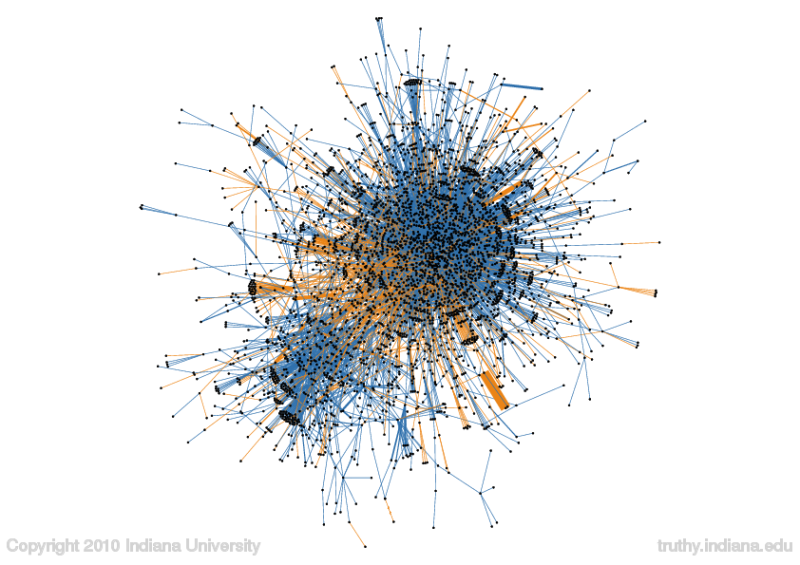
\includegraphics[width=0.9\textwidth]{tcot}
\caption{Diffusion du mème \#tcot sur les réseaux sociaux}
\end{figure}
\\ \\
L'analyse de ces données permet par exemple d'améliorer les résultats des moteurs de recherche, ou encore d'étudier les comportements sociaux. D'autre part, il est intéressant de connaître les comportements des utilisateurs les plus influents, dans le but de comprendre la raison de leur popularité, comprendre ce que leur apporte cette popularité et quels sont leurs buts (en politique par exemple).
\\ \\
Mais les réseaux ne sont pas limités aux réseaux sociaux, et peuvent faire leur apparition dans de multiples domaines : les transports, l'organisation hiérarchique d'une entreprise, les espaces géographiques, les connexions entres les neurones d'un cerveau, ou encore les interactions entre les protéines d'un composé chimique ou biologique. Tant de domaines qui cherchent pourtant des réponses communes.
\begin{figure}[h]
\centering
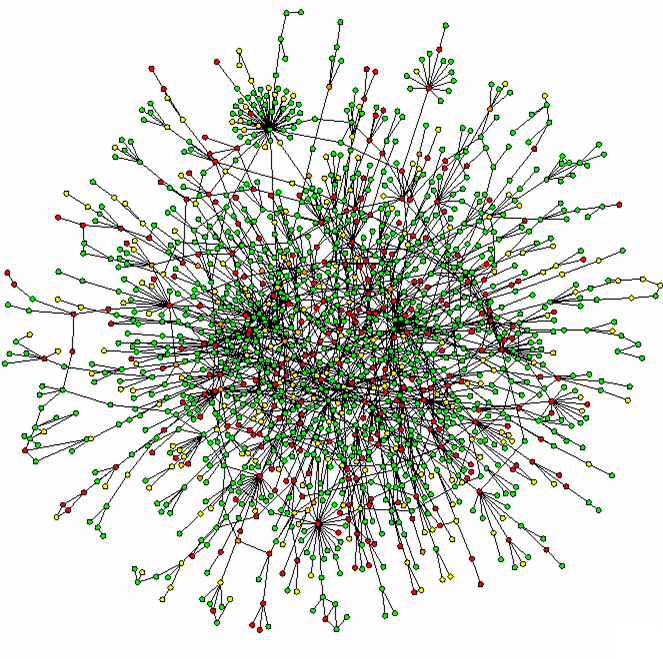
\includegraphics[width=0.9\textwidth]{biology}
\caption{Interactions de protéines dans le Saccharomyces cerevisiae, une levure}
\end{figure}
\\ \\
Dans un premier temps, il est nécessaire de définir quelques concepts liés à la représentation de réseaux sous forme de graphes.
Un graphe est un ensemble de points, dont certaines paires sont directement reliées par un (ou plusieurs) lien(s). Ces liens peuvent être orientés, c'est-à-dire qu'un lien entre deux points u et v relie soit u vers v, soit v vers u : dans ce cas, le graphe est dit orienté. Sinon, les liens sont symétriques, et le graphe est dit non orienté. Afin de représenter au mieux les données, nous pouvons placer des poids sur les noeuds ou sur les arêtes, par exemple : dans un graphe représentant des villes, on pourrait mettre une valeur en kilomètres sur les liens séparants 2 villes ; ou encore affecter le nombre d'habitants d'une ville à chaque noeud correspondant. Le degré d'un noeud correspond au nombre de ses voisins. On définit comme voisins d'un noeud N l'ensemble des noeuds ayant un lien direct avec N. 
\\ \\
Grâce à cela, il est déjà possible de répondre à certaines questions, comme par exemple trouver le chemin le plus court entre deux noeuds. Ou encore, de répondre à des problèmes comme le voyageur de commerce : on se place dans un graphe à n noeuds où l'on connaît les distances séparant chaque noeuds, trouver un chemin de longueur totale minimale qui passe exactement une fois par chaque noeuds et revienne au noeud de départ. L'ensemble des algorithmes de la théorie des graphes nous sert donc comme base pour nos algorithmes d'études de réseaux.
\\ \\ 
Dans un second temps, la théorie des réseaux complexes définit plusieurs mesures comme le nombre de sauts (utilisé dans les réseaux internet pour compter le nombre d'intermédiaire pour aller d'un point à un autre), ou encore la distribution des degrés, c'est à dire la probabilité qu'un noeud, choisi de manière aléatoire, comporte un certain degré. Le degré de séparation est également une notion importante qui définit le nombre de noeuds minimum pour aller d'un noeud à un autre.
\begin{figure}[h]
\centering
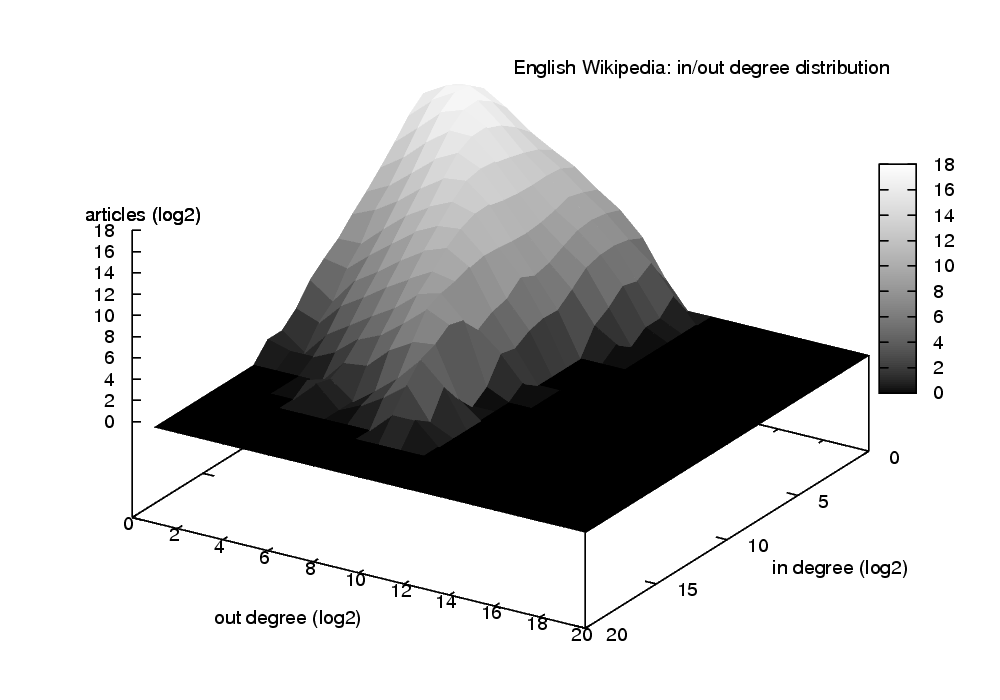
\includegraphics[width=0.9\textwidth]{degreedistribution}
\caption{Exemple de la représentation de la distribution des degrés d'un graphe}
\end{figure}
\\ \\ 
Nous avons vu précédemment qu'avec la théorie des réseaux complexes, on recherche à comprendre comment les réseaux se forment, grandissent, et quelles caractéristiques ils partagent. Nous allons donc décrire plusieurs caractéristiques que les réseaux peuvent avoir en commun.
\\ \\ 
Un réseau est appelé small-world, en référence au phénomène du même nom qui indique que dans un graphe représentant un réseau social, il y a au plus $k$ (avec $k$ petit, souvent inférieur à $10$) degrés de séparation entre deux noeuds. L'idée est donc que, dans un réseau small-world, le degré de séparation entre deux noeuds est très petit (mathématiquement, il augmente de manière logarithmique en fonction de la taille du réseau).
\\ \\ 
Il existe également les réseaux appelés scale-free, dont la distribution des degrés suit une loi de puissance. Une loi de puissance est une relation entre deux quantités x et y qui peut s'écrire de la façon suivante :
$ y = ax^k $
De part la loi de puissance et son principe d'in-variance d'échelle, les réseaux scale-free suivent cette propriété de loi de puissance peu importe l'échelle du graphe (nombre de noeuds/liens).
\\ \\ 
Nous pouvons être amenés à vouloir partitionner un ensemble d'utilisateurs, afin d'observer les groupes d'individus ayant une liaison forte (ces groupes sont appelés communautés~\cite{communautes, structure}). Grâce à ce que nous avons vu, nous pouvons par exemple essayer de savoir quels noeuds du réseau sont importants, influents, centraux, ou connaitre quel contenu recommander à quelqu'un dont on connaît les goûts de ses amis, ou de sa communauté.
}

%------------------------------Fin Introduction------------------------------
%------------------------------Analyse de l'existant------------------------------

\newpage
\begin{center}
\begin{bf}
\section{Analyse de l'existant}
\end{bf}
\end{center}

\vspace{1cm}
{
Actuellement, une partie des algorithmes que nous allons reprendre a déjà été implémentée, notre travail va donc consister à adapter ces algorithmes pour notre structure de données, et à implémenter nous-mêmes les algorithmes restants. 
Les al\=gorithmes que nous allons devoir traiter sont les suivants : \\ \\
	
\begin{description}
\item[Jaccard :] Il s'agit d'étudier le jaccard \cite{jaccard} de deux ensembles de sommets A et B, c'est à dire le cardinal de l'intersection de A et B, divisé par le cardinal de l'union de A et B. A est l'ensemble des voisins sortants et B l'ensemble des voisins entrants. \[J(A,B) = \frac{|A \cap B|}{|A \cup B|}\] Cela permet de voir les similitudes en deux ensembles. Par exemple, on peut comparer le voisinage de deux utilisateurs et déterminer leur ressemblance, ou encore comparer les communautés résultantes d'algorithmes différents afin de voir  leur correspondance. Il existe aussi OverlapIndex qui permet de mesurer le chevauchement de deux ensembles et est défini comme ceci : \[O(A,B) = \frac{|A \cap B|}{min(|A|,|B|)}\]
\item[K-core~\cite{alvarezhamelin} :] On cherche à obtenir un sous graphe maximal induit $G_{max}$, tel que chacun des degrés des nœuds de $G_{max}$ soit supérieur ou égal à K dans $G_{max}$. C'est la définition d'un sous graphe dense par l'assouplissement de la définition d'une clique (tous les sommets d'une clique sont deux-à-deux adjacents) car les cliques sont peu présentes dans les réseaux. On constate en général que dans des processus de diffusion d'informations, celle-ci se fait au sein d'un même core, du k le plus élevé vers le plus petit.
\newline
\item[Louvain :] Pour faire simple, on étudie avec cet algorithme la comparaison entre le fait que deux éléments  soient connectés, et leur probabilité de l'être. C'est grâce à cela qu'on peut détecter des communautés. On utilise donc la modularité pour que chaque nœud appartienne à une seule communauté. La modularité est définie par: \[\Delta=\sum_{i\,j}\left[ A_{i\,j}-\frac{d_i d_j}{2^m}\right] \delta\left(c_i , c_j \right)\] où $A_{i\,j}$ est la matrice d'adjacence, $\frac{d_i d_j}{2^m}$ est la probabilité de i et j d'être connectés et $\delta(c_i , c_j)$ le fait ou non que i et j soit dans la même communauté.

\newpage
\begin{figure}[ht]
\centering
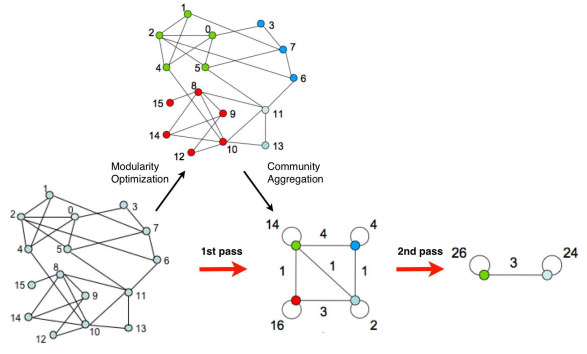
\includegraphics[width=0.9\textwidth]{fast}
\caption{Un exemple des différentes étapes de l'algorithme de Louvain}
\end{figure}
\item[Guimera et Amaral :]  On se penchera ici sur le rôle que jouent les nœuds, c'est à dire s'ils sont hubs (s'ils sont incontournables dans une communauté), ce qui est définit par le z-score de leur degré interne (le nombre de noeuds de la m\^eme communauté auquel un noeud est connecté. Empiriquement, un hub est dit hub si ce score est supérieur à 2.5. On étudie également la connectivité d'un noeud aux autres communautés à travers la participation externe. Un noeud est dit connecteur s'il est connecté à  beaucoup d'autres communautés. En revanche, il est dit périphérique s'il dispose de peu de connexions vers d'autres communautés que la sienne). Le z-score est défini comme suit: \[Z_i=\frac{l_i-\overline{L}}{\sigma_L}\] où $L = \{l_i,...,l_n\} $ avec $l$ les liaisons du nœud actuel, $L$ la moyenne des liaisons des nœuds de la communauté et $\sigma$ l'écart type. Le z-score du degré interne est la normalisation entre les différents graphes. Il permet d'obtenir le nombre de liaisons dans la communauté  proportionnellement aux liaisons des autres nœuds de la communauté.\[Z_i=\frac{d_{int}^i - \overline{d_{int}^{c_i}}}{\sigma_{d_{int}}^{c_i}}\] La participation externe permet de connaître la connectivité avec l'extérieur (vers 0 quand peu connecté avec l'extérieur, vers 1 quand très connecté). \[P_i=\sum_i\left(\frac{d_c}{d_i}\right)^2\] $d_c$ est le degré du noeud i dans sa communauté.\cite{GA}
\newline
\item[Dugué et Perez  :] Ce dernier point est une adaptation des mesures de Guimera et Amaral. On traitera de la connectivité externe, en étudiant la diversité, l'intensité et l'hétérogénéité. La diversité correspond au z-score du nombre de communautés externes auquel le noeud est connecté. L'intensité correspond au z-score du nombre de liens vers l'extérieur. Enfin, l'hétérogénéité est l'écart type de la moyenne des liens vers les communautés extérieures, par communauté extérieure, et pour chaque nœud. \cite{NDAP1}\cite{NDAP2} 
\end{description}


D'autre part, les algorithmes déjà codés sont répartis de manière éparse sur différents fichiers, et il n'y a aucune cohésion entre eux ; notre travail va donc être de rassembler toutes les fonctionnalités de manière organisée, d'en faire une librairie.
}

%------------------------------Fin Analyse de l'existant------------------------------
%------------------------------Besoins non fonctionnels------------------------------

\newpage
\begin{center}
\begin{bf}
\section{Besoins non fonctionnels}
\end{bf}
\end{center}

\vspace{1cm}
{
Ce qui est attendu de nous pour ces travaux, c'est de débuter la constitution d'une librairie, comportant tous les algorithmes abordés précédemment, qui simplifierait leur utilisation de manière uniformisée et par conséquent simplifierait l'étude des grands graphes.
\\ \\ 
}

\subsection{Choix du langage}
{
\textbf{Description :} Notre bibliothèque devra être développée en C++.

\textbf{Priorité :} 10/10

\textbf{Justification :} Les solutions existantes sont déjà en C++. De plus, les programmes qui utilisent les solutions existantes le sont également. Enfin, cela permet un usage simple dans des programmes en C++. Par ailleurs, C++ est un language performant et OpenMP permet de paralléliser simplement du code C++ . Ainsi, par souci de continuité et de performance, C++ est choisi
}

\subsection{Environnement cible}
\subsubsection{La machine Speed}
{
\textbf{Description :} L'environnement cible de notre bibliothèque est la machine Speed qui comporte 64 coeurs et 64 Go de RAM. En outre l'utilisation de la mémoire doit être limité.

\textbf{Priorité :} 10/10

\textbf{Justification :} Avec 64Go et des réseaux qui peuvent en occuper la moitié, il est nécessaire d'avoir des algorithmes n'abusant pas de la mémoire vive.
}

\subsubsection{Algorithmes non-récursif}
{
\textbf{Description :} On tentera d'éviter au maximum l'utilisation d'algorithme récursif.

\textbf{Priorité :} 9/10

\textbf{Justification :} Les graphes peuvent comporter un très grand nombre de noeuds et de sommets (plusieurs millions de noeuds), il est donc important de ne pas utiliser d'algorithme récursif sur le nombre de noeuds par exemple. En effet, la pile d'appel de fonctions pourrait ne pas pouvoir contenir l'ensemble de nos appels récursif et ferait donc planter l'exécution de notre programme avec une erreur de type \textit{StackOverflow}.
}

\subsection{Performance}
\subsubsection{Utilisation de la mémoire vive}
{
\textbf{Description :} L'environnement cible comporte 64 Go de RAM, son utilisation est donc limité. Néanmoins, il est nécessaire de savoir l'utiliser intelligemment.

\textbf{Priorité :} 10/10

\textbf{Justification :} En effet, bien qu'étant une ressource précieuse, la RAM peut nous aider à améliorer les performances en temps de nos algorithmes. En outre, si stocker certaines informations en mémoire (sans en abuser) lors de l'utilisation d'un algorithme permet d'augmenter sensiblement sa rapidité d'exécution, alors il est important d'étudier si le gain en temps vaut le sacrifice en mémoire.
}

\subsubsection{Temps de calcul}
{
\textbf{Description :} Les algorithmes ne doivent pas nécessiter une exécution de plus de quelques heures sur des réseaux tels que Twitter, sans compter la parallélisation.

\textbf{Priorité :} 10/10

\textbf{Justification :} Étant donné la quantité d'informations à traiter et le nombre de personnes utilisant la machine Speed, il est nécessaire de restreindre son temps d'utilisation.
}

\subsection{Mise en place d'une bibliothèque dynamique}
{
\textbf{Description :} Si possible, nous pourrions mettre en place une librairie dynamique sous forme de .DLL (Windows) et .so (Linux). \cite{dll1}\cite{dll2}\cite{dll3} Dans le cas contraire, la bibliothèque sera utilisées comme les solutions existantes, c'est à dire comme un ensemble de fichier .h et .cpp (fichier template et code source de C++).

\textbf{Priorité :} 1/10

\textbf{Justification :} Une bibliothèque dynamique permet de regrouper l'ensemble d'une bibliothèque de fonctions sous un seul fichier (.dll ou .so). Permettant une distribution facilitée de la bibliothèque à une tierce personne. De plus, cela permet d'avoir une seule instance de la bibliothèque qui s'exécute et répond aux demandes en temps réel.
}

%------------------------------Fin Besoins non fonctionnels------------------------------
%------------------------------Besoins fonctionnels------------------------------

\newpage
\begin{center}
\begin{bf}
\section{Besoins fonctionnels}
\end{bf}
\end{center}

\subsection{Code}

\subsubsection{Pattern}
{
\textbf{Description :} Utilisation de design pattern.

\textbf{Priorité :} 10/10

\textbf{Justification :} La librairie sur laquelle nous travaillons doit pouvoir être enrichie par la suite, et ce facilement, sans avoir à se plonger dans le code. Le principe du design pattern est de penser la conception d'un programme, l'organisation des classes le composant, de manière à pouvoir intégrer très aisément de nouveaux composants, à travers une structure du code modulaire.
}

\subsubsection{Parallélisation}
{
\textbf{Description :} Afin d'améliorer le temps d'exécution de nos algorithmes, nous utiliserons OpenMP \cite{OpenMP}  sur les algorithmes les plus gourmands en temps.

\textbf{Priorité :} 9/10

\textbf{Justification :} En effet, l'environnement cible dispose de 64 coeurs, il est donc très intéressant de paralléliser nos programmes et de bénéficier d'un temps de calculs beaucoup plus réduit. OpenMP \cite{OpenMP} permet une parallélisation simple de programmes grâce à l'utilisation de directives (lignes de code qui seront remplacées à la compilation pour transformer certains blocs en blocs parallèles, avec des paramètres définis).
}

\subsection{Algorithmes}

\subsubsection{BFS}
{
\textbf{Description :} Breadth First Search, ou algorithme de parcours en largeur. \cite{BFS}

\textbf{Priorité :} 10/10

\textbf{Justification :} Cet algorithme permet le parcours d'un graphe de manière itérative, à l'aide d'une structure de type file. Nos algorithmes suivants requièrent pour la plupart à un moment ou à un autre de parcourir le graphe à étudier, cet algorithme est donc fondamental.
}

\subsubsection{Jaccard}
{
\textbf{Description :} Permet de connaître le jaccard \cite{jaccard} de deux ensembles.

\textbf{Priorité :} 9/10

\textbf{Justification :} Comme on l'a vu précédemment, le jaccard \cite{jaccard} permet la comparaison de deux ensembles, cet algorithme est donc un élément essentiel puisqu'utilisé par plusieurs autres algorithmes.
}

\subsubsection{K-core}
{
\textbf{Description :} Obtention d'un sous graphe de type K-core

\textbf{Priorité :} 9/10

\textbf{Justification :} Il permet d'étudier la diffusion d'informations et les noyaux centraux qui les diffusent, et est lui aussi utilisé par d'autres algorithmes.
}

\subsubsection{Louvain}
{
\textbf{Description :} Comparaison entre le fait que deux objets soit connectés et leur probabilité de l'être.

\textbf{Priorité :} 8/10

\textbf{Justification :} Cet algorithme permet de détecter des communautés, son appartenance à la librairie est capitale, même si sa priorité n'est pas absolue du fait qu'il ne soit pas utilisé dans la plupart des autres algorithmes.
}

\subsubsection{Guimera et Amaral}
{
\textbf{Description :} Le rôle des nœuds.

\textbf{Priorité :} 7/10

\textbf{Justification :} Pour étudier un graphe, il est important de connaître l'importance de chaque nœud au sein de sa communauté comme au sein des autres communautés. Il est donc fort utile de disposer de cet algorithme dans notre librairie, mais, pour autant, peu d'algorithmes risquent d'avoir besoin de celui-ci.
}

\subsubsection{Dugué et Perez }
{
\textbf{Description :} Adaptation des mesures de Guimera et Amaral.

\textbf{Priorité :} 6/10

\textbf{Justification :} Cet algorithme servira pour traiter la connectivité externe, à travers la diversité, l'intensité et l'hétérogénéité. De même que Guimera et Amaral, cet algorithme sera beaucoup utilisé pour étudier les graphes, mais ne sera pas intégré à d'autres algorithmes.
}

\subsection{Tests}

{
\textbf{Description :} Réalisation de tests.

\textbf{Priorité :} 8/10

\textbf{Justification :} Lorsque l'on écrit un programme, il est nécéssaire de de vérifier qu'il fonctionne ; pour cela on réalise des tests. Ces tests permettent de s'assurer que le code ne bug pas, qu'il réalise ce pourquoi il a été écrit, et qu"il ne fait rien d'autre que cela. Il est donc vital pour notre librairie de tester notre code.
}

\subsection{Documentation}

{
\textbf{Description :} Ajout de documentation au code.

\textbf{Priorité :} 10/10

\textbf{Justification :} De manière à rendre un code compréhensible par toutes les personnes ayant à le relire, que ce soit pour ceux qui l'écrivent au départ ou pour ceux qui le reprendront, il est important de bien le documenter : de la sorte sa compréhension sera facilitée.
}

\vspace{1cm}
\subsection{Prototype papier}

\begin{figure}[h]
\centering
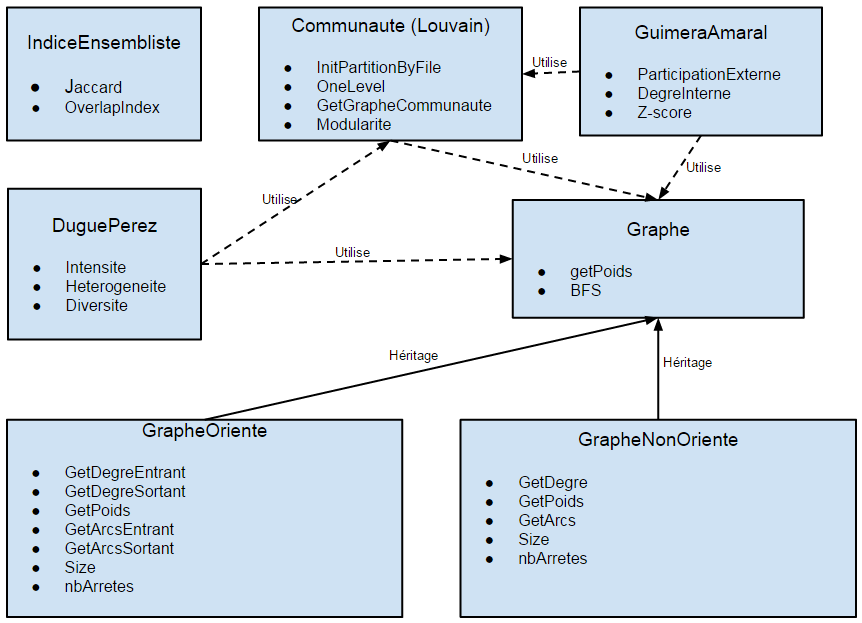
\includegraphics[width=0.99\textwidth]{proto0}
\caption{Prototype papier de la bibliothèque}
\end{figure}

{
La librairie que nous allons constituer devra rassembler l'ensemble des algorithmes que nous serons à même de retranscrire depuis la solution existante, c'est à dire l'ensemble des algorithmes vus précédemment. Mais elle devra également comporter des algorithmes de base de la théorie des graphes, tels que le parcours en largeur ou en profondeur. L'objectif est d'avoir une librairie suffisamment flexible et modulaire, afin que de nombreux algorithmes puissent être ajoutés et cela même après la fin de ce TER.
\\ \\ 
C'est pourquoi il est essentiel de mettre en place un modèle permettant de représenter un graphe, qu'il soit orienté ou non, de pouvoir convertir un graphe orienté en non-orienté. Ou encore, de pouvoir utiliser un graphe de la même manière qu'il soit orienté ou non, ce qui peut être utile dans des algorithmes qui ne se préoccupent pas de l'orientation. En outre, il est important de pouvoir spécifier si une fonction prend en paramètre uniquement un graphe orienté, non-orienté ou les deux.
\\ \\ 
Afin de faciliter l'utilisation de la librairie, nous avons effectué des recherches sur la mise en place d'une librairie dynamique. Ceci permet de pouvoir facilement partager le code présent dans la librairie pour de multiples exécutions, et ce sans avoir accès à l'implémentation de la librairie, facilitant ainsi la distribution de cette dernière auprès de tierces personnes. Pour autant, les difficultés liées aux environnements de développement multiples (Linux avec l'extension .so, et Windows avec l'extension .dll), nous amèneraient à passer du temps sur une fonctionnalité non-essentielle, temps qui pourrait être mieux investi.
\\ \\ 
C'est pour cette raison que la librairie sera constituée de multiples fichiers .cpp et .h, comme c'est le cas de la solution existante. En effet, cela permet une utilisation simple et rapide de l'ensemble de la librairie pour l'écriture d'un nouveau projet de manipulation de graphe, et ce, peu importe l'environnement de développement ou d'exécution. C'est également un moyen permettant plus de libertés quant à l'enrichissement de cette librairie.
\\ \\ 
L'utilisation de cette librairie s'effectuera par l'inclusion des bons fichier header (\#include "Graphe.h"), et l'utilisation des fonctions et classes sera aussi aisé que l'utilisation de classes et fonctions d'un projet en cours. Bien évidement, aucune interface graphique n'est demandée, puisque le but est de fournir un ensemble d'outils (classes et fonctions) permettant la mise en oeuvre simple, rapide et uniforme de nouveaux projets/solutions pour le traitement des graphes importants sur super-calculateurs.
}

%------------------------------Fin Besoins fonctionnels------------------------------
%------------------------------Prototypes et resultats de tests------------------------------

\newpage
\begin{center}
\begin{bf}
\section{Prototypes et résultats de tests}
\end{bf}
\end{center}

\vspace{1cm}
{
Nous avons dans un premier temps commencé par coder la structure de données.
Étant donnée la taille importante des graphes à stocker en mémoire, il nous fallait un moyen d'avoir un accès direct à un sommet ainsi que ses voisins. La méthode utilisée est donc la suivante : trois tableaux distincts. 
\\ \\
•     Un pour stocker les arcs entrants d'un sommet
\\ \\
•     Un autre pour les arcs sortants
\\ \\
•     Un dernier permettant de savoir, pour chaque sommet, où regarder dans les deux autres tableaux afin d'avoir les voisins correspondants. 
\\ \\
Cela nous permet d'avoir un temps constant lors de la recherche des voisins, car on n'a pas à parcourir toute la liste des sommets, et chaque sommet n'est stocké en mémoire qu'une fois.
\\ \\
Pour représenter ces tableaux nous avons utilisé les "vector" présents en C++, car cela nous permet un accès direct aux données dans le tableau (contrairement aux listes par exemple, où le get fait un parcours de la liste) et d'avoir un tableau dynamique.
\\ \\
Une fois ceci fait, nous n'avons pu tester notre structure de données que sur de petits graphes, loin de la taille des graphes pour lesquels notre programme doit tourner, car ce sont des graphes prenant plusieurs dizaines de Go de mémoire. 
\\ \\
Heureusement, la taille des graphes en mémoire n'est pas importante car il vaut mieux tester nos algorithmes sur un graphe faible en mémoire, plutôt que sur un de 25 Go, car le temps d'exécution et donc le temps de debug sera ainsi beaucoup plus court.
}

%------------------------------Fin Prototypes et resultats de tests------------------------------
%------------------------------Planning et affectation des taches------------------------------

\newpage
\begin{center}
\begin{bf}
\section{Planning et affectation des taches}
\end{bf}
\end{center}

\vspace{1cm}
{
Pour mener à bien ce travail, nous prenons contact avec Nicolas Dugué une fois par semaine, pour faire le point sur nos avancées et définir ou redéfinir des objectifs. Nous utilisons un dépôt svn pour gérer les fichiers, et l'outil Trello pour nous répartir les tâches.
\begin{figure}[h]
\centering
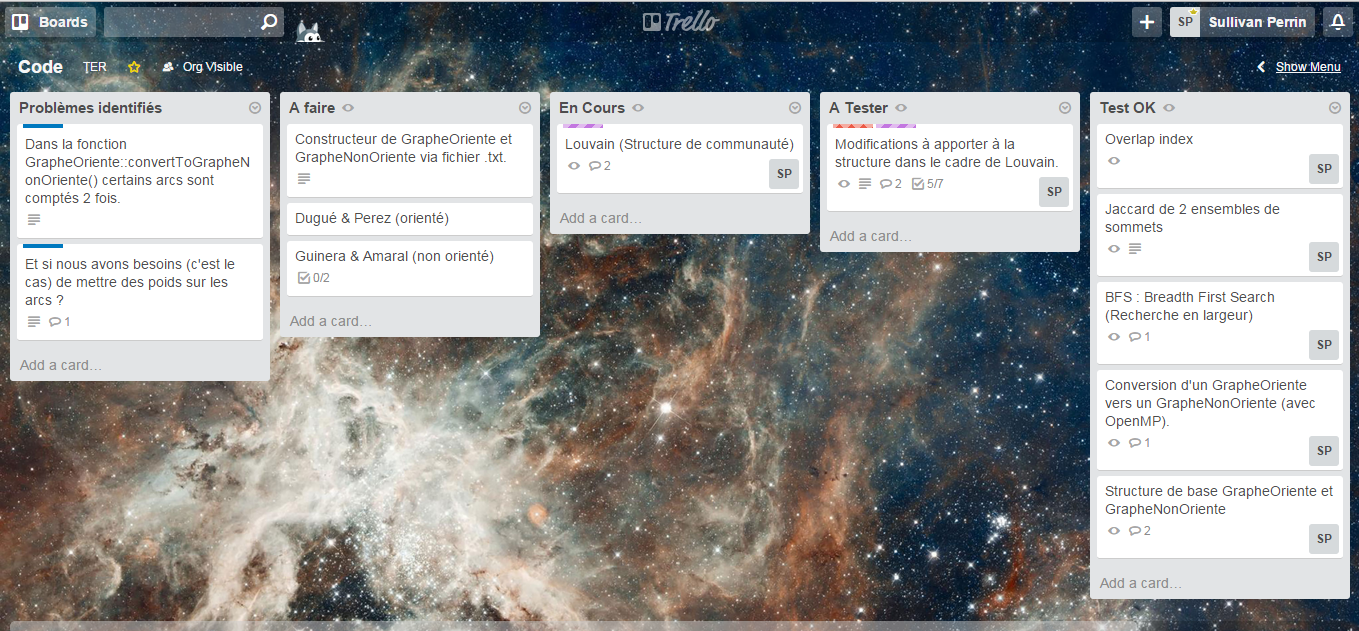
\includegraphics[width=0.99\textwidth]{trello}
\caption{Notre page d'organisation sur Trello}
\end{figure}
\\ \\
Nous avons cinq algorithmes principaux à implémenter, mais les cinq n'ont pas la même complexité ; nous essayons donc de chacun travailler sur l'un des algorithmes, tout en faisant régulièrement le point pour pouvoir venir en aide à l'un ou l'autre si une difficulté est rencontrée. Si cette difficulté nous dépasse, nous n'hésiterons pas à faire appel à Nicolas Dugué et/ou à Anthony Perez.
\\ \\
Notre objectif est d'avancer progressivement, de construire notre librairie brique par brique, dans l'optique de la mener le plus loin possible, le mieux possible.
}

%------------------------------Fin Planning et affectation des taches------------------------------

\end{titlepage}